\documentclass[12pt]{article}
\usepackage[a4paper,margin=2.5cm]{geometry}
\usepackage{newtxtext}
\usepackage{libertine}
\usepackage{inconsolata}
\usepackage{nicefrac}
\usepackage[libertine,cmintegrals,cmbraces]{newtxmath}
\usepackage[T1]{fontenc}
\usepackage[small,compact]{titlesec}
\usepackage{natbib}
\usepackage{color}
\usepackage{graphicx}
\usepackage{cancel}
\usepackage[pdftex,colorlinks=true,%
   urlcolor=blue,
   linkcolor=blue,
   citecolor=blue,
   filecolor=blue]{hyperref}
\usepackage{comment}
\usepackage{amsmath}
\usepackage{amssymb}
\usepackage{textcomp}
\usepackage{stmaryrd}
%\usepackage{bm}
% 
% package relsize: needed only if you use \mathlarger, \mathsmaller!!!
%\usepackage{relsize}
%
\def\Xint#1{\mathchoice
{\XXint\displaystyle\textstyle{#1}}%
{\XXint\textstyle\scriptstyle{#1}}%
{\XXint\scriptstyle\scriptscriptstyle{#1}}%
{\XXint\scriptscriptstyle\scriptscriptstyle{#1}}%
\!\int}
\def\XXint#1#2#3{{\setbox0=\hbox{$#1{#2#3}{\int}$}
\vcenter{\hbox{$#2#3$}}\kern-.5\wd0}}
\def\ddashint{\Xint=}
\def\dashint{\Xint-}

% ---------------------------------------------------------------------------
% use Euler Fonts for my own devious ends
% ---------------------------------------------------------------------------
\DeclareMathAlphabet\EuScript{U}{eus}{m}{n}
\SetMathAlphabet\EuScript{bold}{U}{eus}{b}{n}


\newcommand{\bbxfamily}{\fontencoding{U}\fontfamily{bbold}\selectfont}
\newcommand{\textbbx}[1]{{\bbxfamily#1}}
\DeclareMathAlphabet{\mathbbx}{U}{bbold}{m}{n}
\DeclareMathAlphabet{\mathpzc}{OT1}{pzc}{m}{it}
\newcommand{\zapf}{\fontencoding{OT1}\fontfamily{pzc}\fontseries{m}\fontshape{it}\fontsize{16}{16pt}\selectfont}
% ---------------------------------------------------------------------------
% math.tex was originally developed as a set of TeX macros.  Here, it
% is being modified for LaTeX use, so you wil find a mix of TeX and
% LaTeX commands (sorry...).  At any rate, it provides some useful
% macros.  Take a look
%
% Nelson Lu\'{\i}s Dias
% 15 apr 1994
% 27 sep 1996
% 27 sep 2002
% ---------------------------------------------------------------------------
%\newcounter{ItemNumber} %
% ---------------------------------------------------------------------------
% the fourier-transform of long expressions is typed as a wide hat after
% the expression
% ---------------------------------------------------------------------------
\newcommand{\aft}{\widehat{\phantom{u}}}
% ---------------------------------------------------------------------------
% macros to simplify math typing
% ---------------------------------------------------------------------------
\DeclareMathOperator{\sen}{sen}%
\DeclareMathOperator{\senh}{senh}%
\DeclareMathOperator{\tg}{tg}%
\DeclareMathOperator{\tgh}{tgh}%
\DeclareMathOperator{\cotgh}{cotgh}%
\DeclareMathOperator{\snl}{snl}
\DeclareMathOperator{\arcsen}{arcsen}%
\DeclareMathOperator{\erf}{erf}%
\DeclareMathOperator{\erfc}{erfc}%
\DeclareMathOperator{\haversin}{haversin}%
\DeclareMathOperator{\arcsenh}{arcsenh}%
\DeclareMathOperator{\arctg}{arctg}%
\DeclareMathOperator{\arctgyx}{arctg2}%
\DeclareMathOperator{\cis}{cis}%
\newcommand{\arctgh}{{\rm arctgh}}%
\newcommand{\blob}{\; \mbox{\rule{4pt}{4pt}}}%
\newcommand{\bfvec}[1]{\mathord{\mbox{\bf #1}}}%
\newcommand{\cotg}{{\rm cotg\,}}%
\newcommand{\cross}{\vet{\times}}
\newcommand{\deriva}[2]{\frac{d{#1}}{d{#2}}}%
\newcommand{\mderiva}[2]{\frac{\md{#1}}{\md{#2}}}%
\def\dbar{{\raisebox{-0.75pt}{$\mathchar'26$}\mkern-14.5mu\mathrm{d}}} 
\newcommand{\dimof}[1]{\left\llbracket #1 \right\rrbracket}
\DeclareMathOperator{\Cov}{Cov}%
\DeclareMathOperator{\Var}{Var}%
\DeclareMathOperator{\MSE}{MSE}
\DeclareMathOperator{\RMSE}{RMSE}
\DeclareMathOperator{\EMQ}{EMQ}%
\DeclareMathOperator{\REMQ}{REMQ}
\DeclareMathOperator{\Exv}{E}%
\DeclareMathOperator{\Co}{Co}
\DeclareMathOperator{\Qu}{Qu}
\DeclareMathOperator{\Rea}{Re}
\DeclareMathOperator{\Img}{Im}
% ----------------------------------------------------------------------------
% \derder must be considered obsolete, but is kept for backward compatibility;
% \dern is preferable
% ----------------------------------------------------------------------------
\newcommand{\derder}[3]{%
   \frac{d^{#3}{#1}}
        {d{#2}^{#3}}
}%
\newcommand{\dern}[3]{%
   \frac{d^{#3}{#1}}
        {d{#2}^{#3}}
}%
\newcommand{\mdern}[3]{%
   \frac{\md^{#3}{#1}}
        {\md{#2}^{#3}}
}%
\newcommand{\dmat}[1]{\frac{ D{#1}}{Dt}}%
\newcommand{\dmatbar}[1]{\frac{ \overline{D}{#1}}{Dt}}%
\newcommand{\fof}[1]{\mathord{\mbox{\large\it ff}\,{(#1)}}}%
\newcommand{\ifonlyif}{{\; \Leftrightarrow \;}}%
\providecommand{\implies}{\; \Rightarrow \;}%
\newcommand{\then}{\; \Rightarrow \;}%
\newcommand{\parder}[2]{ {\frac{\partial {#1}}{\partial{#2}} }}%
\newcommand{\thermopar}[3]{{\left(\frac{\partial {#1}}{\partial{#2}}\right)_{#3} }}%

\newcommand{\parpar}[3]{\frac{\partial^2 {#1}}{\partial{#2} \partial{#3}}}%
\newcommand{\parparpar}[4]{\frac{\partial^3 {#1}}{\partial{#2} \partial{#3}\partial{#4}}}%
\newcommand{\parn}[3]{%
    \frac{\partial^{#3} {#1}}%
         {\partial {#2}^{#3}}
}%
\newcommand{\parpow}[2]{ {\left( #1 \right) }^{#2} }%
\newcommand{\such}{\;|\;}%
\newcommand{\totder}[2]{ {D{#1} \over D{#2} } }%
\newcommand{\ulvec}[1]{\underline{#1}}
%\def\well#1{\mathstrut #1}%
%\def\I{\, \mathord{\sl i}\, }%
% ---------------------------------------------------------
% the classic sets
% ---------------------------------------------------------
\newcommand{\rea}{\mathbb{R}}%
\newcommand{\com}{\mathbb{C}}%
\newcommand{\reb}{\mathbb{R}^2}%
\newcommand{\ren}{\mathbb{R}^n}
% ---------------------------------------------------------
% math formulas, displaystyle, in LR mode
% ---------------------------------------------------------
\newcommand{\mathbox}[1]{%
\mbox{$\displaystyle #1$}%
}
\newcommand{\tavg}[1]{\left\langle #1 \right\rangle}
\newcommand{\tavh}[1]{\langle #1 \rangle}
% -----------------------------------------------------------------------------
% e e i
% -----------------------------------------------------------------------------
\newcommand{\me}{\mathrm{e}}
\newcommand{\mi}{\mathrm{i}}
\newcommand{\md}{\mathrm{d}}
%% \newcommand{\md}{\mathord{\textsl{d}}}
%% \newcommand{\mi}{\mathord{\textsl{i}}\,}
%% \newcommand{\me}{\mathord{\textsl{e}}}

% ---------------------------------------------------------------
% minha redefini��o local de vetor
% ---------------------------------------------------------------
%\newcommand{\vet}[1]{\mathbf{#1}}
\newcommand{\bdot}{\boldsymbol{\cdot}}
\newcommand{\vet}[1]{\boldsymbol{#1}}
\newcommand{\vut}[1]{\ensuremath{\mathbf{#1}}}
\newcommand{\vem}[1]{\underset{\sim}{#1}}
\newcommand{\ven}[1]{\underset{\approx}{#1}}
\newcommand{\veg}[1]{\mathord{\mbox{\boldmath $#1$}}}
%\newcommand{\mat}[1]{\mathord{[\mbox{\boldmath $#1$}]}}
%\newcommand{\met}[1]{\mathord{\mbox{\boldmath $[#1]$}}}
\newcommand{\met}[1]{\mbox{$\boldsymbol{[}$} \boldsymbol{#1} \mbox{$\boldsymbol{]}$}}
\newcommand{\mat}[1]{\mbox{$\boldsymbol{[}$} #1 \mbox{$\boldsymbol{]}$}}
\newcommand{\mut}[1]{\ensuremath{\mathbf{[#1]}}}
% --------------------------------------------------------------------
% mathptmx requires a special treatment
% --------------------------------------------------------------------
%\newcommand{\mut}[1]{\mathord{\mbox{       $\bm{[#1]}$}}}
% --------------------------------------------------------------------
% 
% --------------------------------------------------------------------
\newcommand{\bigmat}[1]{\mbox{$\boldsymbol{\big[}$} #1 \mbox{$\boldsymbol{\big]}$}}
\newcommand{\Bigmat}[1]{\mbox{$\boldsymbol{\Big[}$} #1 \mbox{$\boldsymbol{\Big]}$}}
\newcommand{\biggmat}[1]{\mbox{$\boldsymbol{\bigg[}$} #1 \mbox{$\boldsymbol{\bigg]}$}}
\newcommand{\Biggmat}[1]{\mbox{$\boldsymbol{\Bigg[}$} #1 \mbox{$\boldsymbol{\Bigg]}$}}
\newcommand{\ten}[1]{\mathbb{#1}}
\newcommand{\mlin}[1]{[#1]^{\mathsf{\small T}}}
%\newcommand{\tr} {{\mbox{\tiny$\mathsf{T}$}}}
\newcommand{\tr} {{\mbox{\tiny$\boldsymbol{\top}$}}}
\newcommand{\adj}{{\mbox{\tiny$\dagger$}}}
\newcommand{\tuplet}[1]{({#1}_1,{#1}_2,{#1}_3)}
\newcommand{\tuplen}[1]{({#1}_1,{#1}_2,\ldots,{#1}_n)}
\newcommand{\jac}[2]{\frac{\partial\tuplen{#1}}{\partial\tuplen{#2}}}
% -----------------------------------------------------------------------------
% latitude, longitude
% -----------------------------------------------------------------------------
\newcommand{\latmin}[3]{#1\textdegree\,#2\textquotesingle\,#3}
\newcommand{\lonmin}[3]{#1\textdegree\,#2\textquotesingle\,#3}
% -----------------------------------------------------------------------------
% � fun��o de/ n�o � fun��o de
% -----------------------------------------------------------------------------
%\newcommand{\isfunc}[1]{\mbox{=\textflorin}(#1)}
\newcommand{\isfunc}[1]{:=\text{f{\kern-0.1em}f}(#1)}
\newcommand{\isnotfunc}[1]{:\ne\text{f{\kern-0.1em}f}(#1)}
\newcommand{\isconst}[1]{:=\text{\textcent}}
\newcommand{\inner}[2]{\langle {#1},{#2} \rangle}
% ---------------------------------------------------------------------------
% macros to produce uppercase greek letters
% ---------------------------------------------------------------------------
\newcommand{\Alpha}{\mathord{\mathcal{A}}}
\newcommand{\Beta}{\mathord{\mathcal{B}}}
\newcommand{\Epsilon}{\mathord{\mathscr{E}}}
\newcommand{\Zeta}{\mathord{\mathcal{Z}}}
\newcommand{\Eta}{\mathord{\mathcal{H}}}
\newcommand{\Iota}{\mathord{\mathcal{I}}}
\newcommand{\Kappa}{\mathord{\mathcal{K}}}
\newcommand{\Mu}{\mathord{\mathcal{M}}}
\newcommand{\Nu}{\mathord{\mathcal{N}}}
% \newcommand{\omicron}{\mathord{o}}
\newcommand{\Omicron}{\mathord{\mathcal{O}}}
%\newcommand{\Rho}{\mathord{\large\mbox{$\wp$}}}
%\newcommand{\Rho}{\mathord{\mbox{\large{$\wp\!$}}}}
%\newcommand{\Rho}{{\mbox{\large{$\wp{\kern -.1em}$}}}}
% ---------------------------------------------------------------------------
% I don't know how to do this with \newcommand
% ---------------------------------------------------------------------------
\def\Rho{%
\mathchoice%
      {\mbox{\large{$\wp\kern-0.05em$}}}
      {\mbox{\large{$\wp$}}}
      {\scriptstyle\wp}
      {\scriptscriptstyle\wp}
}



% \newcommand{\Rho}{\mathord{\mathcal{P}}}
\newcommand{\Tau}{\mathord{\mathcal{T}}}
\newcommand{\Chi}{\mathord{\mathcal{X}}}
%%\newcommand{\tet}{\mathord{\mbox{\footnotesize$\mathpzc{T}$}}}
\newcommand{\tet}{\mathord{\mbox{\footnotesize$\EuScript{T}$}}}
%%\newcommand{\vsp}{\mathord{\mbox{$\mathscr{V}$}}}
\newcommand{\vsp}{\mathord{\mbox{\small$\mathpzc{V}$}}}
\newcommand{\Ein}{\EuScript{U}}
\newcommand{\Hel}{\EuScript{F}}
\newcommand{\Gib}{\EuScript{G}}

%% -----------------------------------------------------------------------------
%% neat trick!
%% -----------------------------------------------------------------------------
%%\newcommand{\sfbTheta}{\text{{\biolinumGlyph{uni0398}}}}
%%\newcommand{\varRho}{\text{{\libertineGlyph{uni01A4}}}}



%% \newcommand{\Alpha}{\mathord{\mbox{\zapf{A}}}}
%% \newcommand{\Beta}{\mathord{\mbox{\zapf{B}}}}
%% \newcommand{\Epsilon}{\mathord{\mbox{\zapf{E}}}}
%% \newcommand{\Zeta}{\mathord{\mbox{\zapf{Z}}}}
%% \newcommand{\Eta}{\mathord{\mbox{\zapf{H}}}}
%% \newcommand{\Iota}{\mathord{\mbox{\zapf{I}}}}
%% \newcommand{\Kappa}{\mathord{\mbox{\zapf{K}}}}
%% \newcommand{\Mu}{\mathord{\mbox{\zapf{M}}}}
%% \newcommand{\Nu}{\mathord{\mbox{\zapf{N}}}}
%% \newcommand{\omicron}{\mathord{\mbox{\zapf{o}}}}
%% \newcommand{\Omicron}{\mathord{\mbox{\zapf{O}}}}
%% %%\newcommand{\Rho}{\mathord{\mbox{\zapf{P}\,}}}
%% \newcommand{\Rho}{\mbox{\Large$\wp$}}
%% \newcommand{\Tau}{\mathord{\mbox{\zapf{T}}}}
%% \newcommand{\Chi}{\mathord{\mbox{\zapf{X}}}}


% ---------------------------------------------------------------------------
% macros to produce punctuation inside math mode
% ---------------------------------------------------------------------------
%\newcommand{\MathPeriod}{\;{\rm .}}
%\newcommand{\MathComma}{\;{\rm ,}}
%\newcommand{\MathSemiColon}{\;{\rm ;}}
%\newcommand{\MathColon}{\;{\rm :}}
% --------------------------------------------------------------------------
% EqnList provides an environment with a list of equations with numbers 
% like 1-a, 1-b, ...  It works ALMOST like the eqnarray 
% environment,
% but preceding each equation you MUST type \EqnItem
% --------------------------------------------------------------------------
%\newcommand{\EqnItem}{%
%   \addtocounter{ItemNumber}{1}%
%   \addtocounter{equation}{-1}%
%}%
%\newenvironment{EqnList}{%
%   \renewcommand{\theequation}%
%   {\arabic{equation}-\alph{ItemNumber}}%
%   \addtocounter{equation}{1}%
%   \begin{eqnarray}%
%}%
%{%
%   \end{eqnarray}%
%   %\addtocounter{equation}{-1}%
%   \setcounter{ItemNumber}{0}%
%   \renewcommand{\theequation}{\arabic{equation}}%
%}%
\newcommand{\mathsci}[1]{\mathord{\mbox{\small\scfamily\itshape #1}}}
\newlength{\equal}\settowidth{\equal}{$\:=\:$}




















\title{Deterministic and stochastic views of turbulence.}
\author{Nelson L Dias}
\date{\textcolor{blue}{Updated on \today}}

\begin{document}

\maketitle

\begin{abstract}
I want to understand the connection between dynamical systems and stochastic processes.
\end{abstract}

\section{Introduction}

This presentation is about two questions that I have always asked myself (and a
few other people), for which I never obtained statisfactory answers:
\begin{enumerate}
   \item Why do we generate random numbers in a computer in a completely
     deterministic way, and still ``get away'' with it?
   \item Why do we take averages and moments of the quantitities in the
     Navier-Stokes and scalar transport equations, and, again,
``get away'' with the statistics?
\end{enumerate}


It turns out that fairly reasonable answers for these questions are available,
even though there is much more open to learning and researching.  The answers
lie in the intertwined fields of \emph{stochastic processes}, \emph{dynamical
  systems}, and \emph{ergodic theory}. 

I am not qualified to talk about those things at any decent level of knowledge
and depth. Therefore, this talk is little more than a sketch of what I can
\emph{glimpse} to be answers.


In the most basic and perhaps brutal sense, it is profitable to \emph{regard}
turbulence data as realizations of an underlying stochastic process:
\begin{itemize}
\item We can do all kinds of statistical manipulations: means, standard
  deviations, covariances, correlation functions, structure functions, spectra.
\item This is in principle no different than modeling streamflow or
  precipitation as stochastic processes, or fluctuations in the stock market.
\end{itemize}

In this very simple approach, statistics is a \emph{tool} used to analyze a very
complicated phenomenon.  Rather than go into its intricacies, we are content
with a statistical description. Therefore, this approach can be called
``pragmatic'': we forfeit any hope of discussing the underlying \emph{nature} of
the phenomenon, and instead use descriptors of its variability: all we want is
to make statements about the probability of finding values related to the
phenomenon within a specified range.

In many cases, such as the throw of a coin or of a die, although we \emph{know}
that there are equations of motion governing the process, we also think that the
complications of the motion and (most often) the initial conditions are so big
that we are justified in \emph{regarding} the outcome as stochastic: see the
nice figure \ref{fig:dice}.  There, the statistical description boils down to
(perhaps) some experiments at actually throwing dice, and then summing up with
the statement that, for a balanced or fair die, we must have:
\begin{align}
P\{ X = 1\} &=
P\{ X = 2\} =
P\{ X = 3\} =\nonumber \\
P\{ X = 4\} &=
P\{ X = 5\} =
P\{ X = 6\} = 1/6. \label{eq:probdice}
\end{align}
Note the slight circular argument here: a fair die is one that lands on each
face with the same probability!  From (\ref{eq:probdice}), then, we can make
statements such as
\begin{align}
\Exv\{ X\} &= \sum_{i=1}^6 \frac{i}{6} = \frac{21}{6} = \frac{7}{2}, \\
\Var\{ X\} &= \sum_{i=1}^6 \left( i - \nicefrac{7}{2}\right)^2\frac{1}{6} = \frac{35}{12}.
\end{align}

At this point, therefore, we identify two completely separated ways to approach
a problem:
\begin{description}
\item[Deterministically,] by solving the equations for its dynamics, and
  analyzing a certain number of results.
\item[Stochastically,] by \emph{not even employing dynamical equations}, and
  proposing instead statistical descriptors, parametric or not, based on which
  probabilistic statements can be made.
\end{description}

\emph{Statistical mechanics}, on the other hand, tries to employ both
approaches: starting with dynamical equations, we try to derive the
probabilistic laws for the phenomenom that somehow are compatible, from the
beginning, with the dynamics.

Most of the successful approaches to turbulence problems are of this ``mixed''
type. Yet, very seldom do we find in the books and papers an explicit
justification for the approach. More specifically, 
\begin{enumerate}
\item We almost never find a direct mention to the \emph{source} of randomness
  in  a statistical mechanical description: it is usually assumed just to ``be there''.
\item We almost never find a justification for treating the outcome of a
  deterministic dynamical system stochastically.  We take averages of the
  equations, in many senses, and ``get used to it''.
\item The emergence of irreversibility and therefore the second law of
  thermodynamics from deterministic and time-reversible equations (such as the
  laws of motion of classical mechanics) remains a mystery.
\end{enumerate}

A complete solution to these shortcomings is not in sight, and in the current
notes we cannot promise really anything: at the end of the day, we will be
essentially back to 1--3 above.  However, we hope to give enough background
here for one to \emph{undertsand} better the shortcomings of our current
approaches to both the deterministic and the stochastic views of turbulence.




\begin{figure}\centering
\includegraphics[width=0.25\textwidth]{dice}
\caption{Physical dice thrown on a table obey the deterministic equations of
  motion: how come the outcome is ``random''?\label{fig:dice}}
\end{figure}

\begin{comment}
But is this enough?

Is a physical coin a good enough surrogate for a zero-one, equal-probability,
random variable?

Is a computer able to generate such surrogates of random variables? On what
basis do we accept computer-generated randomness as ``good enough randomness''?

And equally important: are the Navier-Stokes equations able to generate an
output that is \emph{really} indistinguishable from stochastic?

I should not talk one hour about that: I will try to talk 5 minutes or 7.5
minutes, and then I must move on.  But I should leave the audiences at least a
reasonable number of good enough answers for us to move on confidently with out
statistical tools.
\end{comment}

\section{Cases where we mix up random and deterministic}

\cite{einstein--uber.molekularkinetischen}'s theory of Brownian motion is a good
example. 

\section{Why do we need an axiomatic approach}

Very good discussion in
\begin{center}
\url{http://scientopia.org/blogs/goodmath/2013/08/24/kolmogorovs-axioms-of-probability/}
\end{center}

and

\url{http://www.ma.utexas.edu/users/mks/statmistakes/probability.html}


\section{State space}

So physicists talk about the space state $\Omega$. In our case, the state space
is the whole field of fluid velocities $U_i$, temperature $T$, density $\Rho$,
and pressure $P$ in a region of physical space where the flow takes place.

The time evolution of the system configuration in state space is a really
interesting thing.  Let the state of the system at $t=0$ be $\vet{x}_0 \in
\Omega$. Although mathematicians don't bother, I am assuming that $\vet{x}_0$ is some
kind of vetor in state space. In a discrete-time evolution, the dynamical system
will evolve according to some rule $T: \Omega \rightarrow \Omega$, so that:
\begin{align*}
\vet{x}_1 &= T(\vet{x}_0),\\
\vet{x}_2 &= T(\vet{x}_1) = T(T\vet{x}_0)), \\
\vet{x}_n &= T(T(\ldots T(\vet{x}_0))) = T^n(\vet{x}_0).
\end{align*}

In a continuous-time evolution, we must have
\begin{align*}
T_0(\vet{x}_0) &= \vet{x}_0, \\
T_s(T_t(\vet{x}_0) &= \vet{x}_{s+t} = T_{s+t}(\vet{x}_0).
\end{align*}

The simplest example, and probably the most interesting to us, is the system of
ordinary differential equations
\[
\mderiva{\vet{x}}{t} = \vet{F}(\vet{x},t).
\]
Numerical solutions of partial differential equations, like the Navier-Stokes
equations, can in principle always be cast in this form.

\section{Examples, from  Collet}

Let $\Omega = [0,1]$ and 
\begin{equation}
f(x) = 2x \bmod 1 \label{eq:omeg-2x}
\end{equation}
We can actually write a simple program, and plot the result.  It is shown in
figure \ref{fig:omeg-2x}.

\begin{figure}
\centering
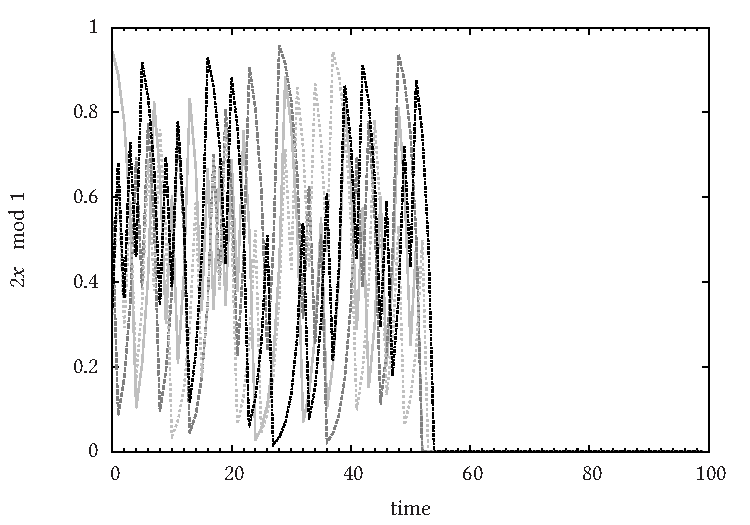
\includegraphics[width=0.6\textwidth]{omeg-2x}
\caption{The dynamical system (\protect\ref{eq:omeg-2x}). For any initial
  condition (4 shown), it locks to 0 after $t \sim 50$.\label{fig:omeg-2x}}
\end{figure}

Our second example is the map
\begin{equation}
f(x) = 16807 x \bmod 2^{31} - 1.  \label{eq:rnum}
\end{equation}
It is shown in figure \ref{fig:rnum}, normalized by $2^{31}$. It is a random
number generator!


\begin{figure}
\centering
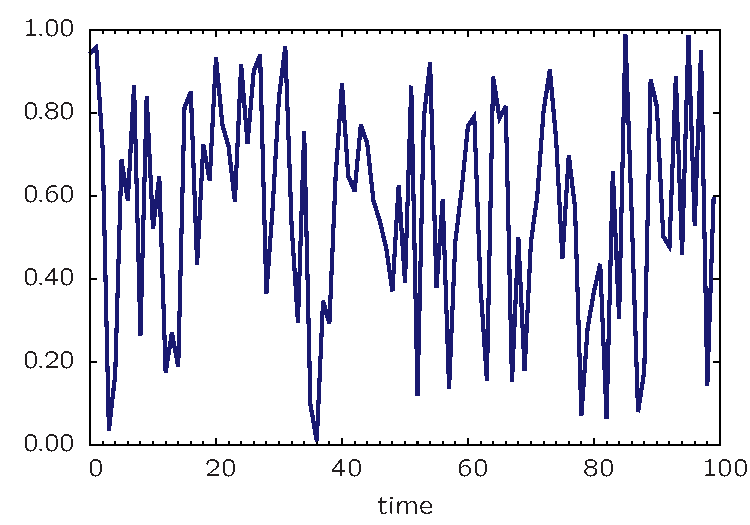
\includegraphics[width=0.6\textwidth]{rnum}
\caption{The dynamical system (\protect\ref{eq:rnum}), a simple random number
  generator.}
\label{fig:rnum}
\end{figure}

In both examples above, $T$ (or $f$) makes $\vet{x}$ re-visit the points of
$\Omega$ on and on. In some loose sense, the relative frequency with which
different regions of $\Omega$ are visited will produce a probability measure on
$\Omega$ (I think).


Then, on p. 8 of Collet: the Navier-Stokes equations are a dynamical system!

So what is the difference between the NS equations and the simple random number
generator (\ref{eq:rnum})?  Maybe not that great!

\begin{verbatim}
Fractional kinetic equations: solutions and applications
BUY: US$ 28,00
RENT: $4.00
Alexander I. Saichev1 and George M. Zaslavsky2
+ VIEW AFFILIATIONS
Chaos 7, 753 (1997); http://dx.doi.org/10.1063/1.166272
\end{verbatim}

According to Collet, there are basically to approaches to understand the time
evolution of a dynamical system:
\begin{description}
\item[The topological, or geometric description,] concerned with orbits,
  attractors, bifurcations, etc.
\item[The ergodic description,] concerned with measures, (and I add:
  probabilities, averages, etc.)
\end{description}

Let us proceed slowly, because Collet is a good source!

Given $A \subset \Omega$, let us define the indicator function $\Chi_A(\vet{x}),
\; \vet{x} \in \Omega$:
\[
\Chi_A(\vet{x}) \equiv \begin{cases}
   1, & \vet{x} \in A, \\
   0, & \vet{x} \not\in A.
\end{cases}
\]
Now let a (discrete-time) dynamical system start at $\vet{x}_0$.  
Note that I don't know whether $\vet{x}_0$ is in $A$.
The average
time that it spends in $A$ until time $N$ is
\begin{equation}
m_N(\vet{x}_0,A) = \frac{1}{N+1}\sum_{j=0}^N \Chi_A(T^j(\vet{x}_0)).
\end{equation}
Then define, assuming its existence:
\begin{equation}
\mu_{\vet{x}_0}(A) = \lim_{N\to\infty} m_N(\vet{x}_0,A). \label{eq:def-mu-x0A}
\end{equation}
First I would like to verify that the limit also exists for $T(\vet{x}_0)$: how
do I do it?


\begin{align*}
m_N(T(\vet{x}_0),A) &= \frac{1}{N+1}\sum_{j=0}^N \Chi_A(T^j(T(\vet{x}_0)))\\
                    &= \frac{1}{N+1}\sum_{j=0}^N \Chi_A(T^{j+1}(\vet{x}_0))
\end{align*}
I want to prove $\mu_{\vet{x}_0}(A) = \mu_{T(\vet{x}_0)}(A)$. I make the
observation that removing finitely many elements from an infinite sum should not
change the limit. Let's try:
\begin{align*}
\mu_{\vet{x}_0}(A) &= \lim_{N\to\infty} \frac{1}{N+1}\sum_{j=0}^N \Chi_A(T^j(\vet{x}_0))\\
                   &= \cancelto{0}{\lim_{N\to\infty} \frac{1}{N+1} \Chi_A(\vet{x}_0)} + 
                      \lim_{N\to\infty} \frac{1}{N+1} \sum_{j=1}^N \Chi_A(T^j(\vet{x}_0))
\end{align*}
In the same vein,
\begin{align*}
\mu_{T(\vet{x}_0})(A) &= \lim_{N\to\infty} \frac{1}{N+1}\sum_{j=0}^N \Chi_A(T^j(T(\vet{x}_0)))\\
                      &= \lim_{N\to\infty} \frac{1}{N+1} \sum_{j=0}^N \Chi_A(T^{j+1}(\vet{x}_0))\\
                      &= \lim_{N\to\infty} \frac{1}{N+1} \sum_{j=1}^N \Chi_A(T^{j}(\vet{x}_0))
                      +   \cancelto{0}{\lim_{N\to\infty} \frac{1}{N+1} \Chi_A(T^{N+1}(\vet{x}_0))}
\end{align*}
Hence, $\mu_{\vet{x}_0}(A) = \mu_{T(\vet{x}_0)}(A)\blob$

Things are bound to become more difficult, however. First, it is \emph{also} OK to write
\begin{align*}
\mu_{\vet{x}_0}(A) &= \lim_{N\to\infty} \frac{1}{N+1}\sum_{j=0}^N \Chi_A(T^j(\vet{x}_0))\\
                   &= \lim_{N\to\infty} \frac{1}{N+1} \sum_{j=0}^{N-1} \Chi_A(T^j(\vet{x}_0))
                   +  \cancelto{0}{\lim_{N\to\infty} \frac{1}{N+1} \Chi_A(T^N(\vet{x}_0))}
\end{align*}
Now,
\begin{align*}
\mu_{T^{-1}(\vet{x}_0)}(A) &= \lim_{N\to\infty} \frac{1}{N+1}\sum_{j=0}^N \Chi_A(T^j(T^{-1}(\vet{x}_0)))\\
                   &= \lim_{N\to\infty} \frac{1}{N+1} \sum_{j=-1}^{N-1} \Chi_A(T^{j}(\vet{x}_0))\\
                   &= \cancelto{0}{\lim_{N\to\infty} \frac{1}{N+1} T^{-1}(\vet{x}_0)} +
                      \lim_{N\to\infty} \frac{1}{N+1} \sum_{j=0}^{N-1} \Chi_A(T^{j}(\vet{x}_0)) = \mu_{\vet{x}_0}(A)\blob
\end{align*}


Now change gear, and look at
\[
m_N(\vet{x}_0,T^{-1}(A)) = \frac{1}{N+1}\sum_{j=0}^N \Chi_{T^{-1}(A)}(T^j(\vet{x}_0)).
\]
The main point here is
\begin{align*}
T^j(\vet{x}_0) \in T^{-1}(A) &\Rightarrow T(T^j(\vet{x}_0)) \in T(T^{-1}(A)),\\
                             &\Rightarrow T^{j+1}(\vet{x}_0) \in A.
\end{align*}
Hence,
\[
\Chi_{T^{-1}(A)}(T^j(\vet{x}_0)) = \Chi_A(T^{j+1}(A).
\]
The fact that $\mu_{\vet{x}_0}(A) = \mu_{\vet{x}_0}(T^{-1}(A))$ follows from the same line of reasoning as above.

From Collet:
\begin{quote}
If one assumes that $\mu_{\vet{x}_0}(A)$ does not depend on $\vet{x}_0$ at least for Borel sets
$A$ (or some other sigma algebra but we will mostly consider the Borel sigma
algebra below), one is immediately lead to the notion of invariant measure.
\end{quote}

A measure $\mu$ on a sigma-algebra $\mathcal{B}$ is invariant by the measurable map $T$ if for any measurable set $A$ 
\begin{equation}
\mu\left(T^{-1}(A)\right) = \mu(A).
\end{equation}
This may be very important!  This may assure that the dynamical system is a ``maker'' of random variables!  Let's find out!

Nomenclature: $(\Omega, T, \mathcal{B}, \mu)$ is a dynamical system with state
space $\Omega$, discrete time evolution $T$, $\mathcal{B}$ is a sigma-algebra on
$\Omega$ such that $T$ is measurable with respect to $\mathcal{B}$ is $\mu$ is a
measure on $\mathcal{B}$ that is invariant by $T$.

\textbf{A broken theorem!}

$\mu$ is invariant if and only if for every measurable $g$ we have 

\begin{equation}
\int g \circ T \,\md{\mu} = \int g \,\md{\mu}.\label{eq:g-on-Omega}
\end{equation}

Now, since $g$ defines a random variable in $\Omega$, the collection $g\circ
T^n$ for all $n$ defines a stochastic process. On account of
(\ref{eq:g-on-Omega}), this is a stationary stochastic process.

\begin{quote}
All the results from the theory of stochastic processes apply to a dynamical
system equipped with an invariant measure.
\end{quote}

It is important to mention that the very notion of what is deterministic, and
what is stochastic, is fuzzy.  For instance, in this passage
\cite{breuer.petruccione--burgers.model}, we read, right at the introduction:
\begin{quote}
It is well known that models of homogeneous turbulence often rely upon
statistical tools [1,2]. In principle, statistical concepts are introduced in
the theory only by considering random initial ensembles of velocity
fields. However, the time evolution of each member is governed by the
deterinistic Navier-Stokes equation.
\end{quote}
In this view, the time evolution is deterministic, and randomness enters via the
initial conditions.  But the general definition of a \emph{stochastic process}
is very similar. It is: given a triplet $(\Omega,\mathcal{F},P)$, a stochastic
process is a \emph{measurable function}
\begin{align*}
   X: (\Omega,T) &\rightarrow \mathbb{R},\\
        (\omega,t)        &\mapsto x = X(\omega,t)
\end{align*}
$T$ is the indexing set. $T$ can be the natural numbers, the integers, the
positive reals, etc.









\bibliography{all}
\bibliographystyle{aaai-named}




\end{document}
